\subsection{Airframe}

\subsection{Propulsion}

\subsection{Flight Control System}
The flight control system on board the UAV encompasses areas such as stability augmentation, navigation, and mission control. These tasks are performed on a completely custom 32-bit ARM-based microcontroller board, which has all required sensors and interfaces directly on it. Additionally, a Raspberry Pi 3+ single-board computer as well the corresponding Pi v2 camera is used for the tasks that require image processing and recognition. A block diagram overview of the entire system is given in Figure \ref{fig:SysBlockDiag} below.

\begin{figure}[H]
\centering
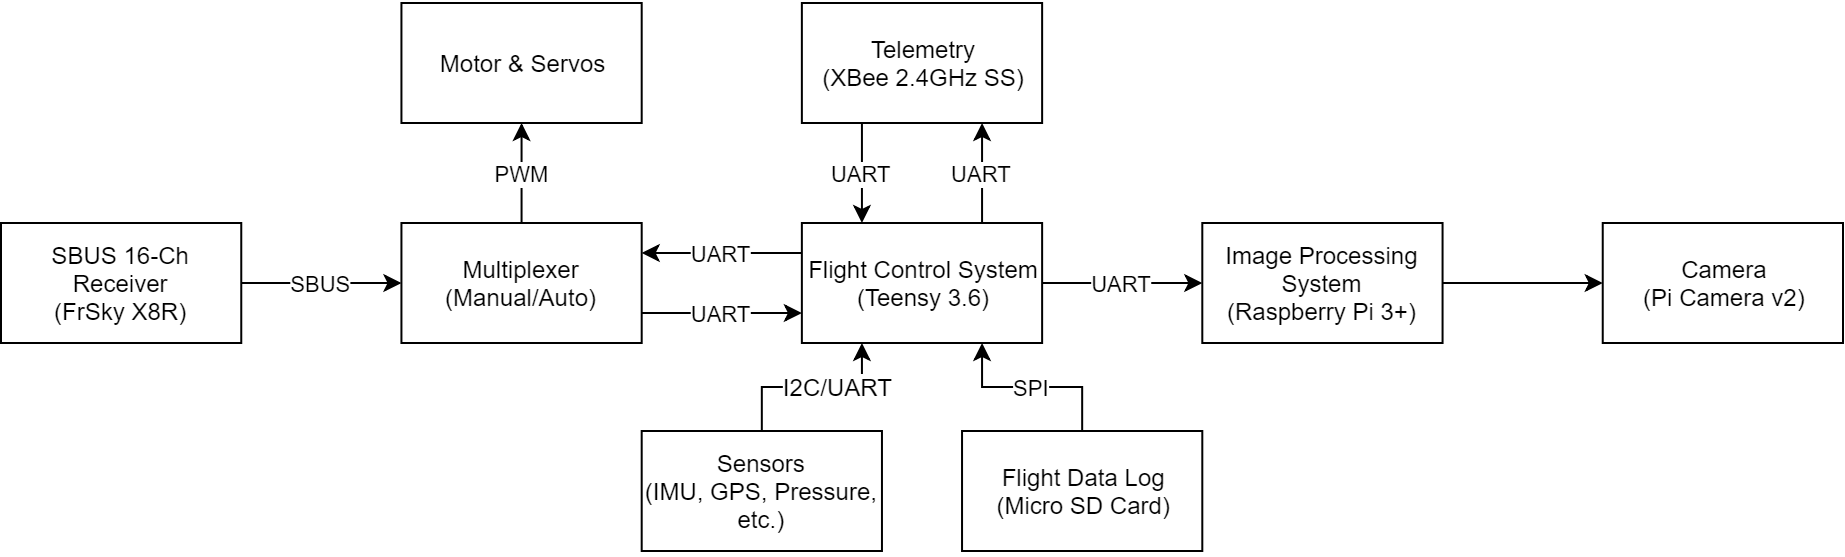
\includegraphics[scale=0.3]{figs/SysBlockDiagram.png}
\caption{System Block Diagram}
\label{fig:SysBlockDiag}
\end{figure}

\subsubsection{Stability}
Closed-loop feedback control is used for stability and provides a robust platform for the higher level autopilots on board the UAV to build on. Feedback is provided from various sensors, e.g. angle of attack, IMU, sideslip (see \textit{Sensor} section below). Dynamic states not directly measurable are estimated using an \textit{Extended Kalman Filter}. \\

The control system was designed using an $H_{\infty}$ loop-shaping approach. This state-of-the-art method of designing control systems combines the classical single-input-single-output (SISO) loop-shaping procedure of classical feedback theory with more modern state-space control, providing benefits of both worlds such as state decoupling, multi-variable feedback, and intuitive setting of closed-loop requirements. Additionally, robustness is guaranteed by giving controllers that meet certain performance specifications even when the system's dynamic model is only approximately known. \\

The UAV's dynamic model was acquired using AVL (DATCOM alternative) which estimates the aerodynamic coefficients and stability derivatives from 3D model data. These coefficients were combined with the equations of motion to give an approximate model of the system with which control design could be performed. \\

\subsubsection{Sensors}
Sensors used for feedback control, as well as higher level features such as GPS navigation, available on the UAV are: \textit{IMU, GPS, Angle of Attack, Sideslip, Camera, Airspeed (Pitot), Barometer, Temperature}.

\subsubsection{Navigation and Mission Control}
Autonomous navigation and mission control is entirely performed on the previously mentioned custom microcontroller board. The system runs as a state machine switching between discrete states as needed, for instance for take-off, reconnaissance, landing, and so forth. The navigation system utilizes the lower-level functionality of the previously described stability augmentation system to set desired roll angles, altitude, airspeed, etc.

\subsection{Image Processing}
The image processing and recognition is performed using a Raspberry Pi 3+ and a Pi v2 camera. The image recognition script is written in Python in combination with the OpenCV library. The system is running constantly, with a description of currently recognised targets being relayed to the main flight control system via a UART serial interface.

\subsection{Innovative Features}
\begin{itemize}
	\item
		innovative feature
\end{itemize}

\subsubsection{Flight Termination System (FTS)}
See section \ref{sec:fts}.

\subsection{Three view drawing}
\vspace*{-0.4cm}
\begin{figure}[H]
	\centering
	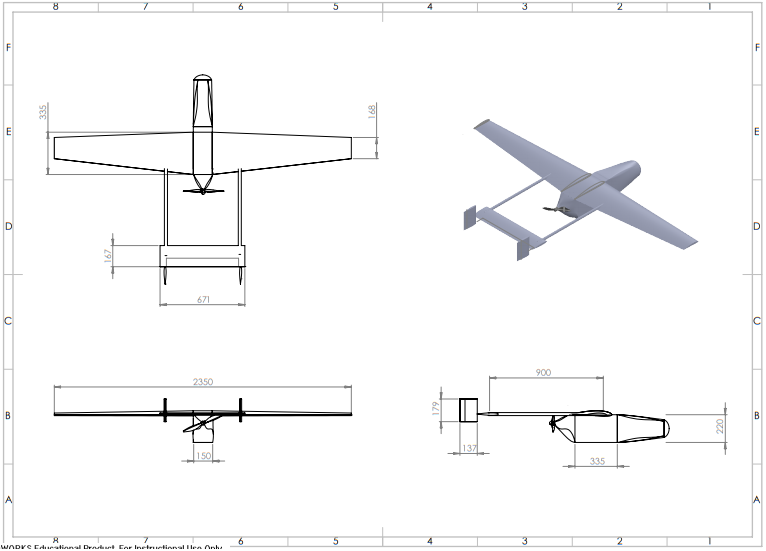
\includegraphics[width=\textwidth]{three_view_drawing}
\end{figure}
